\part{Traiter les données pour la réalisation des projets}

\chapter{Des standards et technologies au service de l'édition numérique}

Les données brutes, bien qu'intéressantes, ne nous permettent pas d'aller bien loin. Une fois que nous avons les transcriptions des correspondances à éditer, il s'agit donc de les traiter pour en assurer la mise en ligne, ce qui est tout l'objet de nos deux projets. Or, que ce soit pour le projet du CRHXIX d'édition numérique de la correspondance de Frédéric Le Play ou pour celui du Labex OBVIL, ELICOM, nous avons eu recours à XML, plus spécifiquement XML-TEI. Ce langage s'avère être en effet particulièrement adapté.

\section{XML, un langage particulièrement approprié}

Comme nous l'avions déjà souligné dans notre deuxième partie, lors de nos réflexions sur l'édition numérique de correspondance\footnote{Voir 4.1.2.3 XML}, XML est un langage structuré, à la fois lisible par l'\oe il humain et par la machine. 

\subsection{XML : présentation générale}
 
\subsubsection{Pourquoi encoder ?}
Le balisage sémantique permet d'expliciter certains aspects du texte\footnote{Voir aussi Elena Pierazzo, \emph{Why do we encode ?} URL : \url{https://www.youtube.com/watch?v=R0ncI_rr1z4&list=PL77mHK9JuenN9NXeXQbVcUORz7HZk-9Pv&index=2} (visité le 04/05/2020). Ce paragraphe s'en inspire.}. L'encodage est très utile pour l'édition car il permet de montrer la structure du texte, ce qu'il est, et non seulement son aspect, sa présentation. Il permet également de séparer le texte et le contenu de l'édition, et donc il permet différents modes d'affichage (notes, transcription normalisée ou non etc.).

Le balisage (\emph{markup}) et l'encodage (\emph{encoding}) n'ont pas été créés avec l'ordinateur, c'est un concept né avec l'imprimerie : en effet, les rédacteurs et éditeurs indiquaient par des symboles comment ils voulaient que le texte apparaisse, quelle taille de caractère, en gras ou en italiques par exemple. De même, la ponctuation et la mise en page sont aussi une sorte de balisage car elles permettent de comprendre comment diviser le texte en segments. Finalement, le balisage, c’est tout ce que nous utilisons pour rendre le texte plus lisible : l’espacement des lettres, les majuscules, le gras, l’italique, la ponctuation. Par ailleurs, encoder est un moyen de veiller à la pérennité des données, à leur conservation sur le long terme.

\subsubsection{Comment encoder ?}

Le langage XML est particulièrement approprié pour nos éditions numériques de correspondance. Il a été créé par le W3C en 1996, avec une contribution importante de la communauté des Humanités Numériques et en particulier de la TEI, comme nous l'avons déjà souligné plus haut.

\inquote{Les données sont incluses dans le document XML sous forme de chaînes de caractères délimitées par un balisage les décrivant. L’unité de base qui comprend données et balisage est appelée élément}\footnote{Voir Ariane Pinche, \emph{Séance 1}, Cours M2 TNAH XML, URL~: \url{https://github.com/ArianePinche/coursTNAH_XML-TEI/blob/master/seance01/InitiationXML.md} (visité le 09/10/2020).}.

Un élément est tout ce qui peut être étiqueté, tout ce qui se décrit, en quelque sorte, tout ce qui est important et devrait être annoté dans le texte.

L'élément a une balise d'ouverture qui se présente avec un chevron (\citecode{<)}), puis le nom du \emph{tag}, le contenu de l'élément puis la balise de fermeture qui a une barre oblique (\citecode{/)} : 

\citecode{<nomElement>chaineCaracteres</nomElement>}

Certains éléments peuvent être vides, dans ce cas on met une barre oblique à la fin : 

\citecode{<nomElement/>}

Les éléments suivent un ordre particulier : soit ils peuvent se suivre les uns après les autres, soit ils s'imbriquent, et dans ce cas, les éléments \emph{enfants} héritent des propriétés des éléments \emph{parents}. Jamais ils ne doivent se chevaucher.

Il faut aussi un élément qui contienne le fichier entier, on l'appelle \inquote{élément racine}.

Les éléments peuvent avoir des attributs, qui servent à préciser quelque chose de l'élément. L'attribut a une syntaxe particulière à respecter~:  après le nom de l’élément, il y a un espace blanc obligatoire, le nom de l'attribut suivi par un signe égal (\citecode{=}) et la valeur de l’attribut est entre guillemets. On peut avoir autant d’attributs qu’on veut dans l'élément mais le même attribut ne peut être utilisé qu’une seule fois\footnote{Pour aller plus loin, voir Ariane Pinche, \emph{ibidem} et les séances. suivantes}.

Un encodage qui respecte ces principes est dit bien formé. 

Par ailleurs, on peut distinguer trois types de balisages\footnote{Nicole Dufournaud, Valérie Gratsac Legendre. \emph{Manuel d’encodage XML-TEI - édition numérique de manuscrits baroques|: Recommandations pour une application TEI}, 2012, Site web HAL, URL~: \url{https://hal.archives-ouvertes.fr/hal-00718043/document} (visité le 28/07/2020).} : 
\begin{itemize}
    \item  Le balisage physique, formel et typographique encode les structures logique et formelle du texte
    \item  Le balisage sémantique autorise un encodage d'un premier niveau d'analyse comme les noms, les toponymes, les citations, les discours et les dates
    \item Le balisage analytique complète l'apparat savant de l'encodage.
\end{itemize}

\subsection{Les métadonnées}

Tout d'abord, pour bien gérer les données, il est important de les décrire au fur et à mesure. Ainsi, \inquote{préalablement à tout encodage, il est nécessaire de donner des informations descriptives et déclaratives sur le texte en vue de sa diffusion, d'un échange de données ou encore de son exploitation : ces composantes – ou métadonnées – forment l'en-tête TEI nommé \citecode{<teiHeader>}\footnote{Nicole Dufournaud, Valérie Gratsac Legendre, in \emph{Ibidem.}, p.7.}}

On entend par métadonnées 
\begin{quote}
    \inquote{les données servant à représenter ou   à décrire d'autres données, ici les deux textes édités. Elles contiennent des informations sur la source d'un document, sa nature, son contenu, sa localisation, son histoire, son statut juridique, etc. Elles remplissent un rôle d'indexation qui facilite l'accès au contenu et améliore la recherche. Elles doivent être normalisées grâce à des standards comme Dublin Core, EAD  (Encoded  Archival Description) par exemple afin de permettre l'interopérabilité et l'échange des données\footnote{\emph{Ibidem.}}.}
\end{quote}

Les métadonnées répondent donc à des standards. Or, la correspondance a ses standards propres : nous avons parlé plus haut du \citecode{<correspDesc>} pensé par le \emph{TEI SIG Correspondence}. Pour nos deux projets, nous avons suivi ces directives.

Par ailleurs, le projet ELICOM nous a éclairé dans le choix des métadonnées pour notre projet du CRHXIX, et nous retrouvons à peu près les mêmes informations, même si nous avons un peu plus détaillé le \citecode{<teiHeader>} pour le CRHXIX, avec notamment l'ajout de balises pour suivre les différentes mises à jour des fichiers XML-TEI.\\

Les métadonnées se trouvent donc dans le \citecode{<teiHeader>} et se subdivisent en un certain nombre de balises.\\

\subsubsection{La description bibliographique du document avec le \citecode{<fileDesc>}}
Tout d'abord, le \citecode{<fileDesc>} contient la description bibliographique du document. Pour ELICOM, il est réduit à deux éléments : \begin{itemize}
    \item le \citecode{<titleStmt>}\footnote{Pour le CRHXIX, nous avons ajouté quelques éléments à l'intérieur du \citecode{<titleStmt>} et du \citecode{<publicationStmt>}, le détail est indiqué dans l'ODD disponible dans les livrables, voir 1.4.2.1.1. Le titleStmt.} : il regroupe les informations sur le titre d’une œuvre et les personnes ou institutions responsables de son contenu intellectuel. C'est ici que sont nommés les principaux responsables du projet pour le CRHXIX. On indique les autres membres de l'équipe et ceux qui ont participé de près ou de loin au projet. Pour chaque personne, on utilise la balise \citecode{<respStmt> }qui englobe la balise \citecode{<resp>}, indiquant la responsabilité qu'a eue la personne en question, la balise \citecode{<name>} qui englobe le prénom puis le nom, et une balise \citecode{<note>} facultative, si jamais l'on a des remarques à faire. La balise \citecode{<note>} peut aussi comprendre un attribut \citecode{@resp} indiquant qui a rédigé la note.
    
    \item le \citecode{<publicationStmt>} : il informe sur la façon dont le projet est distribué ou publié. C'est donc ici qu'est renseignée la licence. Pour l'instant, nous n'avons pas encore déterminé pour le CRHXIX laquelle nous choisissons.
\end{itemize}


Pour le CRHXIX, étant donné que nous travaillons sur des fac-similés, nous y avons en plus ajouté le \citecode{<sourceDesc>}, élément capital pour l'édition numérique de correspondance. En effet, le \citecode{<sourceDesc>}, qui est une description de la source, contient le \citecode{<msDesc>} qui englobe les balises de description du manuscrit, à savoir la balise \citecode{<msIdentifier>} qui elle-même contient la balise \citecode{<country>}. Celle-ci indique le pays d'origine et peut comporter un attribut \citecode{@key} qui est facultatif. La balise \citecode{<settlement>} indique le lieu (ville ou autre), puis on renseigne l' \citecode{<institution>} qui abrite le manuscrit. La balise \citecode{<repository>} contient le nom d'un dépôt dans lequel des manuscrits sont entreposés, et qui peut faire partie d'une institution, et l'\citecode{<idno>} (identifiant) donne un numéro normalisé ou non qui peut être utilisé pour identifier une référence bibliographique.

Pour l'instant, nous ne voyons pas trop l'utilité de la balise \citecode{<msContents>} pour le projet du CRHXIX. Elle renseigne le contenu du manuscrit, décrivant le contenu intellectuel d'un manuscrit ou d'une partie d'un manuscrit, soit en une série de paragraphes \citecode{<p>}, soit sous la forme d'une série d'éléments structurés \citecode{<msItem>} concernant les items du manuscrit. Néanmoins, je laisse la possibilité de l'utiliser, mais on pourrait la supprimer par la suite.

En revanche, la balise \citecode{<physDesc>} pourra s'avérer utile. Elle contient la balise \citecode{<handDesc>} qui mentionne dans le \citecode{<handNote>} quelle main a écrit le manuscrit. Or, si Le Play écrit de sa main la plupart du temps, ce n'est pas toujours le cas, notamment quand il est malade. Pour les autres correspondants, le temps nous a manqué pour nous pencher sur la question, néanmoins, il sera toujours intéressant pour le lecteur non spécialiste et qui ne connaît donc pas les écritures, d'être informé du rédacteur du manuscrit.

\subsubsection{La description détaillée des aspects non bibliographiques avec le \citecode{<profileDesc>}}

Après la description bibliographique du document dans le \citecode{<fileDesc>}, on trouve une description détaillée des aspects non bibliographiques dans le \citecode{<profileDesc>}.

Un des éléments clés qui nous intéresse ici, et qui a été mentionné dans nos deux projets, est le \citecode{<correspDesc>}. Il comprend les informations de description de l'action liée à la correspondance. Celui-ci comprend principalement la balise \citecode{<correspAction>}. Celle-ci se décline en deux temps, selon ses attributs.

\begin{itemize}
    \item Tout d'abord, une balise \citecode{<correspAction>} avec un attribut type comprenant la valeur \citecode{sent} renseigne qui a envoyé la lettre. La balise \citecode{<persName>} comprend donc le prénom puis le nom de l'expéditeur (la plupart du temps il s'agit de Le Play). Elle comprend un attribut \citecode{@key} qui décrit l'expéditeur de façon normalisée et un attribut \citecode{@ref} qui renvoie vers sa fiche data.bnf. La balise \citecode{<settlement>} renseigne le lieu de rédaction de la lettre, et la balise \citecode{<date>} indique la date à laquelle la lettre a été écrite. L'attribut \citecode{@when} permet de la normaliser au format \citecode{AAAA-MM-JJ}. 
    
    \item Puis on retrouve une deuxième balise \citecode{<correspAction>} avec un attribut \citecode{@type} comprenant cette fois la valeur \citecode{received} renseignant à qui la lettre a été envoyée. La balise \citecode{<persName>} comprend donc le prénom puis le nom du destinataire. Elle comprend également un attribut \citecode{@key} qui décrit l'expéditeur de façon normalisée et un attribut \citecode{@ref} qui renvoie vers sa fiche data.bnf. Il y a possibilité d'ajouter une balise \citecode{<settlement>} renseignant le lieu de réception de la lettre, autrement dit le lieu où se trouve le destinataire, et la balise \citecode{<date>} indiquant la date de réception. L'attribut \citecode{@when} permet de la normaliser au format \citecode{AAAA-MM-JJ}. Cependant, il est bien clair que ces deux dernières informations ne seront quasiment jamais renseignées\footnote{Tout au moins c'est l'opinion que l'on peut avoir aujourd'hui, peut-être variera-t-elle dans le temps.}.
\end{itemize}
Ces choix du \citecode{<correspAction>} qui avaient été faits pour ELICOM nous ont donc inspiré pour le projet du CRHXIX.

Toujours dans le \citecode{<correspDesc>} l'on renseigne le \citecode{<correspContext>}, à savoir le contexte dans lequel se situe la lettre, quelle lettre la précède, quelle lettre la suit. On renseigne ces deux informations dans une balise \citecode{<ref>} avec un attribut \citecode{@type} de valeur \citecode{previous} pour la lettre précédente, de valeur \citecode{next} pour la suivante, et on le fait suivre d'un attribut \citecode{@target} qui fait pointer vers le fichier XML en question.

Dans le \citecode{<profileDesc>} se trouve également le \citecode{<settingDesc>} et le \citecode{<particDesc>}. Nous y reviendrons lorsque nous parlerons des index.

\subsubsection{L'historique du fichier avec le \citecode{<revisionDesc>}}
Le dernier élément du \citecode{<teiHeader>} est le \citecode{<revisionDesc>} qui résume l'historique des révisions pour un fichier.

Chaque changement est mentionné sous la balise \citecode{<change>}. Autrement dit, à chaque modification importante du fichier XML, on renseigne quelle modification a été faite (\citecode{<change>}), à quelle date avec l'attribut \citecode{@when}, par qui avec l'attribut \citecode{@who}.


\subsection{XML et le rituel épistolaire}

\subsubsection{Remise en contexte}
Avec XML, nous pourrions en soi encoder le monde entier, avec l'inconvénient sûr de s'y perdre. Il est donc important que le schéma de balise que nous serons amenée à choisir pour nos éditions numériques de correspondance soit le plus restreint possible. 

Par ailleurs, nous avons choisi de répondre aux conseils établis par la communauté scientifique et le TEI P5\footnote{Voir la partie 2 sur penser l'édition et \emph{TEI~: P5 Guideline}, TEI guidelines,  URL~:\url{https://tei-c.org/guidelines/p5/} (visité le 26/09/2020).}. Grâce aux \emph{TEI guidelines}, nous sommes face à des noms d'éléments définis. Il s'agit donc pour nous de suivre les directives du \emph{TEI : Correspondence SIG}. Il n'y a pas de place ici pour la fantaisie. Tout est bien normé. Il suffit simplement de définir quelles balises nous choisissons, et le cas échéant, dans quel ordre nous voulons qu'elles apparaissent.

Or, il faut que notre balisage rende compte des caractéristiques et de la structure propre à la correspondance. Comme nous l'avons vu plus haut, il y a ce qu'on appelle le \inquote{rituel épistolaire\footnote{ Richard Walter (dir.), \emph{L’édition numérique de correspondances – guide méthodologique}, URL :  \url{https://cahier.hypotheses.org/guide-correspondance} (visité le 17/06/2020). Voir particulièrement la page 13.}.}. Voici donc comment il peut se traduire  lorsqu'on encode : 

\begin{itemize}
    \item Le lieu de rédaction et la date apparaîtront en XML-TEI par la ligne \citecode{<dateline>} qui comprend les balises \citecode{<date>} pour la date et \citecode{<place>} pour le lieu
    \item Une \inquote{adresse} ou formule de politesse débutant la lettre, se traduira en balises par \citecode{<salute>}
    \item Une formule de politesse finale sera également transcrite dans un \citecode{<salute>}
    \item Une signature : en général, F. Le Play pour Frédéric Le Play. Si elle n'y est pas, on indiquera qu'elle est manquante, ceci dans la balise \citecode{<signed>}
    \item Éventuellement un post-scriptum qui trouvera sa place dans une balise \citecode{<postscript>}
\end{itemize}

Ainsi, la structure de la lettre est bien mise en évidence. L'encodage répond à nos attentes. Avant de développer le rituel épistolaire, remettons-le dans son contexte.\\

\subsubsection{Le \citecode{<body>}}
Cette structure de la lettre apparaît donc après les métadonnées du \citecode{<teiHeader>},dans la balise \citecode{<text>} qui comprend en général trois éléments : le \citecode{<front>} pour tous les éléments liminaires, le \citecode{<body>} pour le corps du texte proprement dit, le \citecode{<back>} pour tous les appendices, épilogues et postfaces. Pour nos éditions numériques de correspondance, nous développerons surtout la balise \citecode{<body>}.

Celle-ci comprend une division (\citecode{<div>}) avec un attribut \citecode{@type} dont la valeur est \citecode{lettre}. Si la lettre a été rédigée en deux fois, on peut donc utiliser plusieurs \citecode{<div>}, avec un attribut \citecode{@part} dont la valeur sera \citecode{I} pour le début ou partie initiale, \citecode{F} pour la partie finale, \citecode{M} pour le milieu si nécessaire. Cela permettra également d'ajouter une \citecode{<dateline>} pour les autres parties.

La première balise ensuite à mettre dans la \citecode{<div>} - uniquement pour l'édition numérique de la correspondance de Frédéric Le Play cette fois, car cela concerne les fac-similés - est la balise \citecode{<pb>}, qui permet de relier le fichier XML en question avec le manuscrit numérisé. On utilise tout d'abord un attribut \citecode{@n} pour renseigner le numéro du manuscrit, cela va de 1 à l'infini, et on peut y ajouter en plus une lettre en minuscule quand la lettre fait plusieurs pages et donc que le même fichier XML doit être mis en lien avec plusieurs images numérisées. Ainsi, la première page de la lettre 2 est numérotée 2a, la deuxième page 2b, la troisième page 2c et ainsi de suite.

L'attribut \citecode{@facs} pour les fac-similés pointe directement vers une image ou vers une partie d'une image correspondant au contenu de l'élément. On y met comme valeur le nom du fichier image, comme indiqué sur la figure 10.1.

\begin{figure}[ht]
    \centering
    \caption{Capture d'écran de l'ODD du CRHXIX, le \citecode{<pb>}}
    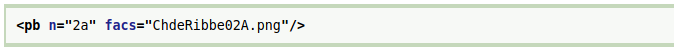
\includegraphics[width=16cm]{images/facs.png}
    \label{facs}
\end{figure}

Dès que l'on change de page de manuscrit au sein du même fichier XML donc de la même lettre, il faut donc à nouveau mettre la balise \citecode{<pb>} pour redonner toutes ces informations, entre la fin de la page précédente et le début de la nouvelle page.

\subsubsection{Le début de la lettre}
La balise \citecode{<opener>} souligne le rituel épistolaire. Elle abrite tous les éléments qui font débuter une lettre, à savoir l'élément \citecode{<dateline>} pour la ligne mentionnant le lieu (\citecode{<placeName>} avec attribut \citecode{@ref}, dont la valeur comprend un \citecode{\#}, pour pointer vers l'index) et la date (\citecode{<date>}) de rédaction de la lettre\footnote{Il faut encore décider si on normalise aussi à cet endroit la date avec un attribut \citecode{@when} ou si c'est inutile étant donné que cela a déjà été fait dans le \citecode{<correspDesc>} du \citecode{<teiHeader>}.}.

Le corps de la lettre nécessite parfois l'emploi d'autres balises pour traiter les cas particuliers\footnote{Encore une fois, ce paragraphe ne concerne que le CRHXIX, étant donné que nous avons affaire à des manuscrits qui n'ont jamais été publiés. La question ne se pose pas pour ELICOM qui travaille sur des éditions imprimées.}. C'est le cas des abréviations. Afin de garder les deux versions\footnote{La question n'a pas encore été tranchée pour le CRHXIX.}, la version originale et la version normalisée, on utilise une balise générale \citecode{<choice>} qui abrite deux balises : la première \citecode{<abbr>} garde l'abréviation originale de l'auteur. La deuxième \citecode{<expan>} donne le mot entier.

Une procédure assez similaire se fait pour la correction des fautes ou la normalisation des lettres. On utilise alors une balise \citecode{<choice>} qui englobe une balise \citecode{<sic>} qui contient le texte original, et une autre \citecode{<corr>} qui contient le texte corrigé.

 \begin{figure}[ht]
    \centering
    \caption{Capture d'écran de l'ODD du CRHXIX, l'\citecode{<opener>}}
    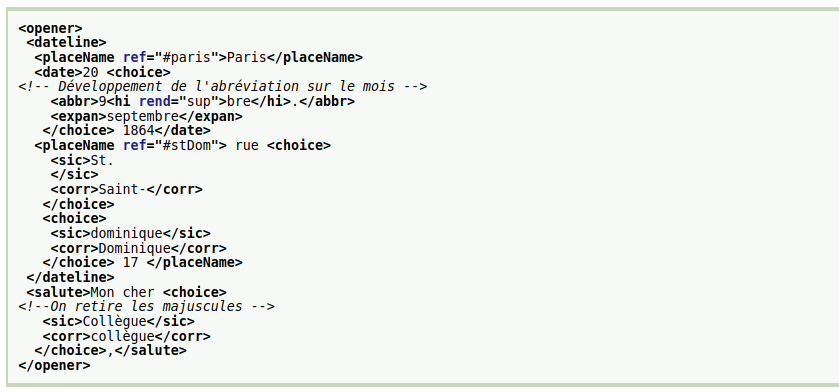
\includegraphics[width=16cm]{images/abbr.png}
    \label{abbr}
\end{figure}

A cela s'ajoute la question du style. Certaines lettres sont en italiques, soulignées etc. Pour manifester ces différents styles, on utilise la balise \citecode{<hi>} avec son attribut \citecode{@rend} qui spécifie la nature du style employé :
\begin{itemize}
    \item \citecode{"italic"} pour les italiques
    \item \citecode{"bold"} si c'est du gras
    \item \citecode{"upper"} pour la mise en capitales du texte sélectionné
    \item \citecode{"small-caps"} pour la mise en petites capitales
    \item \citecode{"sup"} pour la mise en exposant
    \item \citecode{"ul"} pour souligner
    \item \citecode{"line-through"} pour barrer.
\end{itemize}

La balise \citecode{<dateline>} renseignée, il s'agit ensuite de mettre dans la balise \citecode{<salute>} la salutation qui est faite au début de la lettre. Cela fait partie du rituel épistolaire.

Ceci fait, on passe au corps de la lettre.

\subsubsection{Le corps de la lettre}

Le corps de la lettre est contenu dans des balises \citecode{<p>}. Autrement dit, chaque paragraphe est contenu dans une balise \citecode{<p>}. Chaque ligne de ce paragraphe est contenu dans une balise \citecode{<l>}.

Il faut ensuite gérer les cas particuliers. Parfois, l'auteur de la lettre écrit lui-même des notes dans les marges\footnote{Tout ce qui fait référence à la mise en page dans nos dires ne concerne que le CRHXIX. Le reste concerne les deux projets, sauf avis contraire.}. Dans ce cas-là, on peut utiliser une balise \citecode{<note>}. On utilise un attribut \citecode{@resp} pour indiquer que la note a été rédigée par l'auteur de la lettre lui-même, et un attribut \citecode{@place} pour indiquer où la note se trouve dans l'original.

La valeur de l'attribut \citecode{@place} peut varier. Retenons quelques exemples :
\begin{itemize}
    \item \citecode{"above"} : au-dessus de la ligne
    \item \citecode{"below"} : au-dessous de la ligne
    \item \citecode{"bottom} : en bas de page
    \item \citecode{"inline"} : dans le corps du texte
    \item \citecode{"top"} : en haut de page
\end{itemize}

\begin{figure}[ht]
    \centering
    \caption{Capture d'écran de l'ODD du CRHXIX, l'attribut \citecode{@place}}
    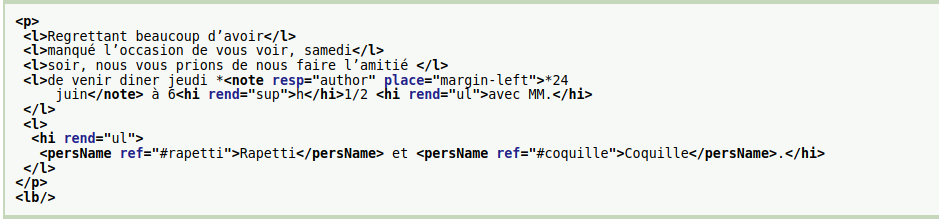
\includegraphics[width=16cm]{images/place.png}
    \label{place}
\end{figure}

Pour le corps de la lettre, nous avons été face à plusieurs questionnements pour ELICOM. En effet, les fichiers XML qui avaient été extraits de l'HTML\footnote{Nous reviendrons tout à l'heure sur cette extraction en parlant rapidement de Python.} comportaient des fautes d'OCR ou d'autres fautes de diverses nature. Par exemple, dans un fichier XML de la correspondance de Félicité de Lamennais, deux fautes sont visibles sur la même page\footnote{Voir Fig. 10.4} : on remarque d'une part un caractère \inquote{i} indiqué à la place d'une marque de crayon à papier. La faute d'interprétation de l'OCR est ici due à la qualité de la numérisation. Un livre usagé a été choisi pour la numérisation ce qui fausse le résultat de l'océrisation. D'autre part, on remarque un problème de guillemets à répétition. En effet, dans l'édition d'origine, les guillemets sont répétés à chaque ligne pour marquer que c'est une citation. Dans notre fichier XML, cela n'a plus de sens car ces guillemets polluent le corps du texte. Certaines modifications et corrections sont donc à apporter au fur et à mesure dans le corps du texte quand cela se présente.

\begin{figure}[ht]
    \centering
    \caption{Des fautes dans un fichier XML (154), Félicité de Lamennais, ELICOM. Capture d'écran d'Oxygen XML Editor et du PDF de l'édition originale.}
    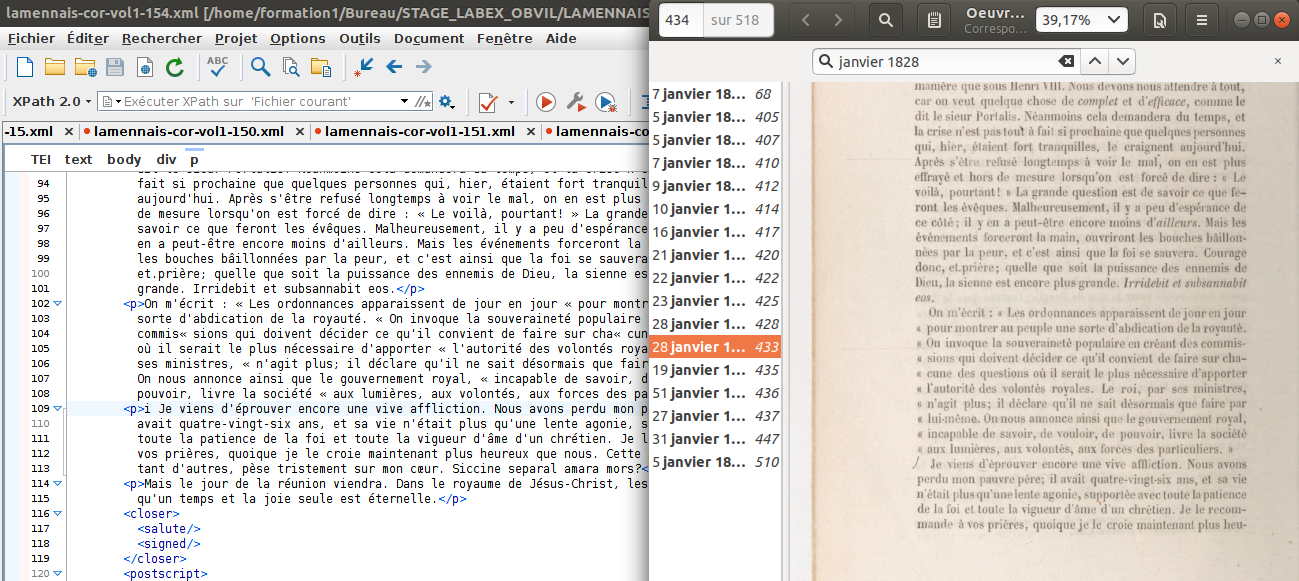
\includegraphics[width=15cm]{images/crayonPapier.png}
    \label{crayonPapier}
\end{figure}

De même, on remarque de faux paragraphes qui se forment ainsi à cause d'un changement de page et qui se doublent d'un tiret séparant le mot. L'ancienne mise en page de l'édition numérique apporte donc des erreurs dans le fichier XML. 

\begin{figure}[ht]
    \centering
    \caption{Faux paragraphes dans un fichier XML (159), Félicité de Lamennais, ELICOM. Capture d'écran d'Oxygen XML Editor et du PDF de l'édition originale.}
    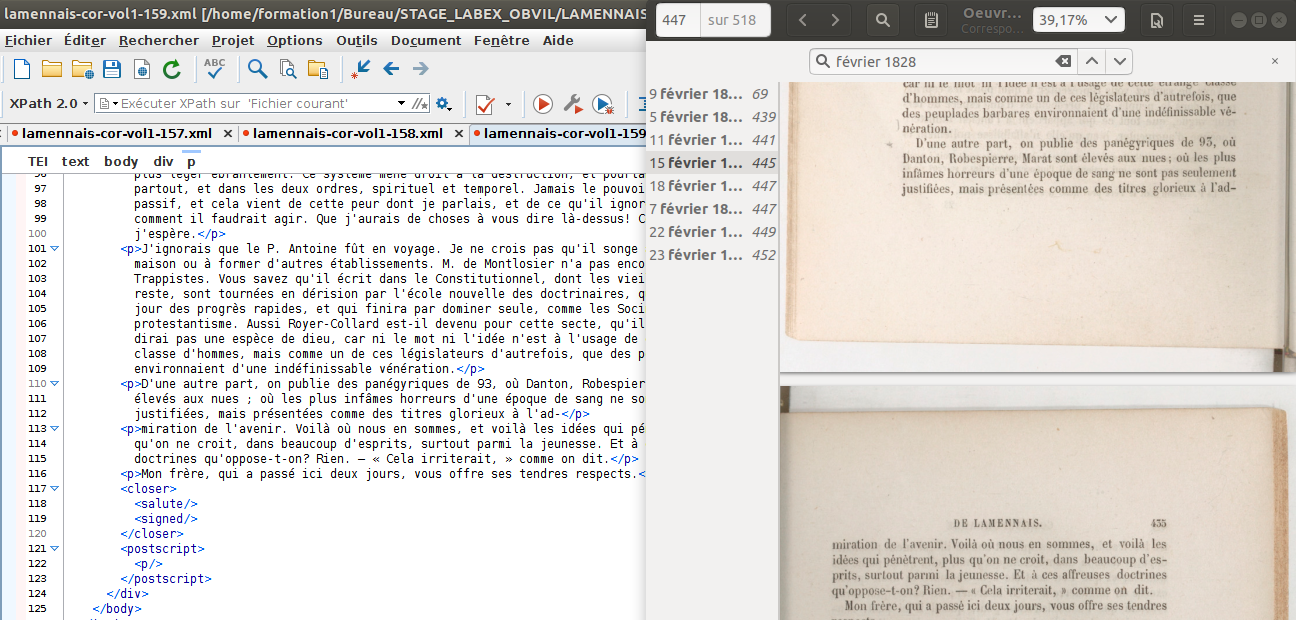
\includegraphics[width=15cm]{images/tirets.png}
    \label{tirets}
\end{figure}

Ainsi, la mise en place et relecture du corps de la lettre a dû être relativement attentive aux problèmes d'océrisation et autres fautes.

\subsubsection{La fin de la lettre}

La balise \citecode{<closer>} marque la fin d'une lettre et fait partie du rituel de correspondance.

Elle-même contient deux balises : d'une part \citecode{<salute>} qui comprend la formule de politesse concluant la lettre, d'autre part \citecode{<signed>} qui englobe la signature. Bien-sûr, la balise \citecode{<salute>} comprend des balises \citecode{<l>} encadrant chaque ligne, c'est toujours le même principe que dans le corps de la lettre. En revanche, les balises \citecode{<p>} ne sont pas admises dans la balise \citecode{<salute>}, probablement parce que les salutations ne font en général pas plus d'un petit paragraphe.

On peut mettre un attribut \citecode{@place} pour indiquer l'emplacement de la signature dans la lettre.

\subsubsection{Le post-scriptum}

La balise \citecode{<postscript>} contient l'éventuel post-scriptum. Elle contient des balises \citecode{<p>} et \citecode{<l>}.
C'est la dernière balise admise dans le corps du texte. Elle achève le fichier XML.

\subsection{Les index}

Par ailleurs, il s'agit de mettre en évidence dans le corps du texte les entités nommées déjà évoquées dans la deuxième partie de notre mémoire\footnote{5.1.2 Cinq dimensions à prendre en compte}. En effet, \inquote{on introduit un balisage dans un document pour l’étiqueter et l’organiser en vue d’un traitement automatisé. Si les paragraphes sont clairement marqués (balisés), alors un logiciel de mise en forme pourra les mettre en page correctement. Si les noms de lieu sont clairement marqués, un programme peut les sélectionner automatiquement pour générer un index géographique\footnote{Lou Burnanrd, \emph{Qu’est-ce que la Text Encoding Initiative~?}, Open Edition Press, 2015, URL~: \url{https://books.openedition.org/oep/1298?lang=fr} (visité le 26/09/2020).}}. Pour ELICOM, nous n'avons pas encore poussé très loin la granularité d'XML : nous avons commencé par transformer les fichiers HTML en fichiers XML sans aller encore très loin dans la description, particulièrement dans le balisage des entités nommées.
En revanche, dans le cadre de l'édition numérique de Le Play, nous nous sommes bien penchée sur la question\footnote{Cette partie sur les index ne concerne donc que le projet d'édition numérique de la correspondance de Frédéric Le PLay.}. Comme annoncé dans la deuxième partie, nous avons choisi d'élaborer six index : index des ouvrages cités, index des événements, index des noms de lieu, des noms de personne, des noms d'organisation, et enfin, index de vocabulaire leplaysien. 


D'une part, dans le corps du texte, à chaque mot indexé, il faut donner la possibilité de pointer vers l'index. Pour les noms de lieu on utilise la balise \citecode{<placeName>}.
\begin{figure}[ht]
    \centering
    \caption{Capture d'écran d'Oxygen XML Editor, pointer vers un index}
    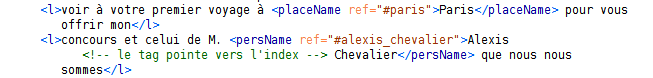
\includegraphics[width=16cm]{images/index.png}
    \label{index}
\end{figure}
Pour les noms de personne ou personnage, on utilise la balise \citecode{<persName>}. Pour les noms d'organisation on utilise la balise \citecode{<orgName>} et pour tous les autres index, on indique la balise \citecode{<name>}. Toutes ces balises ont un attribut \citecode{@ref} qui permet de pointer vers l'index en question avec un tag (\citecode{\#}).



D'autre part, les index en tant que tels se trouvent dans le \citecode{<teiHeader>}. 

\subsubsection{L'index des ouvrages cités}

Dans le \citecode{<sourceDesc>} se trouve un premier index, celui des ouvrages cités dans la correspondance. Tous se situent dans le même index, que ce soient des ouvrages écrits de la main de Le Play ou d'autres contemporains ou antérieurs. Nous avons choisi de renseigner aussi dans cet index les revues et les journaux. Pour les différencier des livres, nous avons pensé à ajouter un attribut \citecode{@type}, qui spécifie si c'est un journal ou une revue.

L'index des ouvrages est englobé dans une balise \citecode{<listBibl>}. Chaque ouvrage (livre, journal ou revue) est contenu dans une balise \citecode{<bibl>}, suivie d'une balise \citecode{<name>} pour le titre, \citecode{<author>} pour l'auteur, \citecode{<date>} normalisée avec l'attribut \citecode{@when}, et une balise \citecode{<note>} est facultative. \begin{figure}[ht]
    \centering
    \caption{Capture d'écran d'Oxygen XML Editor, l'index des ouvrages}
    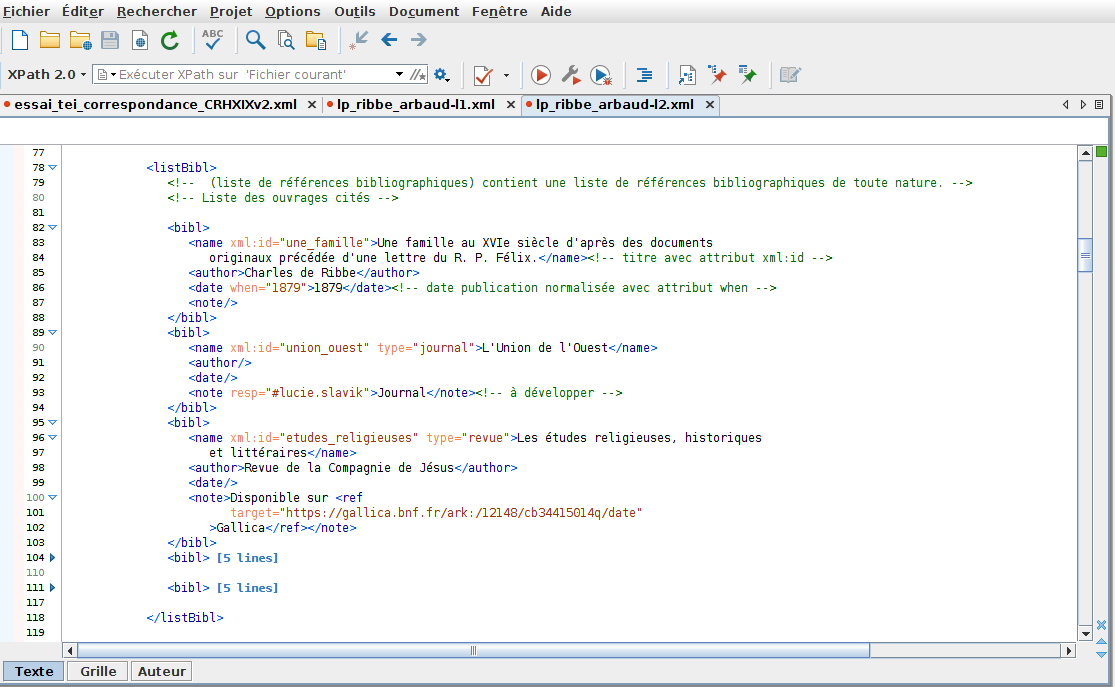
\includegraphics[width=16cm]{images/listBibl.png}
    \label{listBibl}
\end{figure}
À cet endroit, on pourra donner des informations sur l'ouvrage en question. La note pourra comporter un attribut \citecode{@resp} pour indiquer qui en est l'auteur. Cela permettra également de hiérarchiser la qualité des commentaires. Une note rédigée par un étudiant stagiaire sera considérée de moindre valeur que celle d'un spécialiste de Le Play.

La balise \citecode{<name>} doit obligatoirement avoir un attribut \citecode{@xml:id} qui permettra de pointer dans le texte vers l'index.

Par ailleurs, la balise \citecode{<author>} ne sera pas utile pour les journaux. Elle sera donc facultative pour les journaux mais obligatoire pour les ouvrages, distinction qui ne sera pas mentionnée dans l'ODD mais qui est néanmoins importante à avoir en tête.

La balise \citecode{<ref>} avec attribut \citecode{@target} permet de faire un lien vers un site\footnote{À confirmer, nous n'avons pas encore eu l'occasion de le tester.}. 

\subsubsection{L'index des événements}

Toujours dans le \citecode{<sourceDesc>}, après l'index des ouvrages, on trouve l'index des événements, sous la balise \citecode{<listEvent>}. Il recense les événements importants qui sont mentionnés dans la correspondance. Chaque événement marquant est contenu dans une balise \citecode{<event>} avec un attribut \citecode{@when} mentionnant la date normalisée. La balise \citecode{<event>} englobe un \citecode{<label>} contenant le titre de l'événement et comportant un attribut \citecode{@xml:id} indispensable pour qu'on puisse faire référence à l'événement dans le corps du texte. On peut laisser un commentaire sur l'événement dans une balise \citecode{<note>}, avec un attribut \citecode{@resp} indiquant par qui elle a été rédigée.

Les autres index se trouvent dans le \citecode{<profileDesc>}.

\subsubsection{L'index des noms de lieu}
Le \citecode{<settingDesc>} comprend l'index de noms de lieu.
Les informations sur le lieu sont encadrées d'une balise \citecode{<place>} qui a un attribut \citecode{@ xml:id} indispensable pour pointer ensuite du texte vers l'index. Dans le \citecode{<placeName>} est renseigné le nom du lieu, dans \citecode{<country>} le pays, dans la \citecode{<note>}, on peut écrire la description que l'on veut. On peut donc y glisser les notes rédigées par les transcripteurs, ce que nous n'avons pas pris le temps de faire durant les tests d'encodage des premières lettres en XML-TEI. Là encore, il y a possibilité d'y ajouter un attribut \citecode{@resp} pour renseigner qui a écrit la note.


\subsubsection{L'index des noms de personne}

Le \citecode{<particDesc>} (toujours dans le \citecode{<profileDesc>} comprend l'index des noms de personne et personnage mentionnés dans la correspondance. L'index est dans le \citecode{<listPerson>}. 

Pour chaque personne ou personnage, il y a une balise englobante \citecode{<person>} avec un attribut \citecode{@sex} pour indiquer le genre de la personne et un attribut \citecode{@xml:id} indispensable pour lui donner un identifiant qui permettra ensuite dans le texte de pouvoir pointer vers l'index. Le prénom suivi du nom sont indiqués dans la balise \citecode{<persName>}. Une balise \citecode{<note>} permet de présenter la personne en question, mais c'est une présentation générale qui n'est pas liée à une lettre en particulier. Si l'on veut faire une note adaptée à un endroit d'une lettre en particulier, il faut la mettre dans le corps du texte. Pour la \citecode{<note>}, on peut mettre un attribut \citecode{@resp} pour indiquer qui l'a écrite. Pour son contenu, il serait intéressant de réfléchir à une façon plus ou moins normée d'écrire les notes (prénom, nom, titres, dates de naissance et de mort, rôle dans la société en général, avec la sociologie en particulier et lien avec Le Play), ou reprendre tout simplement les normes indiquées par Monsieur Matthieu Brejon de Lavergnée\footnote{Voir 5.2.3 Des choix éditoriaux à faire en amont.}.

\subsubsection{L'index des noms d'organisation}

Le \citecode{<particDesc>} (toujours dans le \citecode{<profileDesc} comprend aussi l'index des noms d'organisation dans le \citecode{<listOrg>}. On peut si l'on veut les regrouper par type d'organisation avec un attribut \citecode{@type}, et faire donc plusieurs index (par exemple, un index d'organisations sociologiques, un index d'organisations politiques, un index d'associations etc.). Mais nous pensons plutôt ne pas faire de distinctions entre les différentes organisations et donc nous limiter à un simple index général pour simplifier au maximum l'encodage, d'autant que le profit retiré ne serait pas si grand.

Le nom de l'organisation est compris dans la balise \citecode{<org>} comprenant l'attribut \citecode{@xml:id} pour son identifiant. La balise \citecode{<orgName>} indique le nom de la société, et la balise \citecode{<note>} (plutôt que \citecode{<desc>}, intialement choisie, mais modifiée dans un souci de simplification) permet de rentrer une note générale sur l'organisation en question.

\subsubsection{L'index leplaysien}

La balise \citecode{<textClass>} comprend tous les autres index. En l'occurrence, il s'agit pour nous de l'index leplaysien. Les mots à indexer sont en cours de choix, la plupart ont été sélectionnés par Messieurs Antoine Savoye, Rémy Hême de Lacotte et Matthieu Brejon de Lavergnée mais il est nécessaire d'y réfléchir encore. Par exemple, nous avons distingué \inquote{ Réforme} de \inquote{Réforme morale} et \inquote{Réforme sociale}. Il serait bon de voir si l'on continue à distinguer ou si l'on met tout sous la même balise, avec le même identifiant \citecode{@xml:id}.

Quoiqu'il en soit, voici comment se présente l'index : on met tout d'abord une balise \citecode{<textClass>} comprenant une balise \citecode{<keywords>} comprenant elle-même une balise \citecode{<list>} avec, pour valeur de l'attribut \citecode{@type}, le nom de l'index dont il est question.

Chaque balise \citecode{<item>} comprend le nom du terme leplaysien avec un attribut \citecode{@xml:id} qui permettra de pointer vers le terme depuis le texte. Une balise \citecode{<note>} permet d'y laisser des commentaires. Il sera possible d'y ajouter un attribut \citecode{@resp} pour indiquer qui en est l'auteur.

Chaque \citecode{<keywords>} ouvrant un index, si l'on avait besoin de faire un autre index, on pourrait le mettre à cet endroit.\\

La réflexion autour de l'indexation a donc été riche. Nous avons d'ailleurs fait appel aux conseils de Monsieur Antoine Savoye, spécialiste de Le Play, pour nous éclairer quant au vocabulaire leplaysien à indexer.

\subsection{La normalisation}

Un des points importants dans XML est la normalisation. Nous l'avons déjà évoqué. Pour ELICOM, nous nous sommes surtout attachée à normaliser, outre les dates (\citecode{AAAA-MM-JJ}), les noms de personne dans le \citecode{<correspAction>}. 

Nous avons repéré en amont les destinataires des différentes correspondances, puis nous avons cherché s'ils étaient présents sur \emph{data.bnf}. En effet, sur \emph{data.bnf}, on trouve des fiches de référence sur les auteurs, les œuvres et les thèmes, et renvoyer à ce site permet l'interopérabilité\footnote{Voir \emph{Accueil}, Site web data.bnf, URL : \url{https://data.bnf.fr/} (visité le 17/06/2020).}.
\begin{figure}[ht]
    \centering
    \caption{La normalisation du \citecode{<correspAction>}, correspondance de Lamartine (\citecode{lamartine-col-vol1-12.xml}), capture d'écran d'Oxygen XML Editor}
    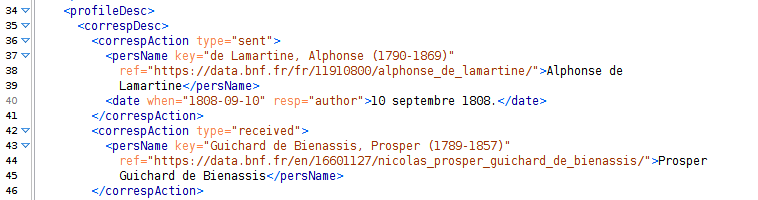
\includegraphics[width=16cm]{images/normalisation.png}
    \label{normalisation}
\end{figure}
Cependant, tous n'étaient pas rencensés dans \emph{data.bnf} notamment parmi les correspondants de Félicité de Lamennais et de Proudhon. Lorsque c'était le cas, nous avons donc supprimé l'attribut \citecode{@ref} renvoyant à \emph{data.bnf} et nous avons mis des parenthèses vides \citecode{(...-...)}, à la place des dates de naissance et de mort, en espérant pouvoir les remplir un jour\footnote{Voir dans les livrables, les dossiers de remarque des différentes correspondances du Labex OBVIL.}.\\


\section{L'ODD et la pérennité des données}

\subsection{Un schéma et une documentation pour la pérennité des données}
Une fois les balises XML définies, il s'agit de créer une documentation dessus pour expliquer nos choix. Or, il existe une technologie qui permet de gérer à la fois le schéma de balises et sa documentation, c'est un document qui fait tout, autrement dit \emph{One document does it all} (ODD).

Tout d'abord, comme le souligne Lou Burnard, \inquote{l'ODD est le langage de définition et de maintenance du système TEI. Il permet la maintenance du code et de sa documentation d’une manière intégrée, à partir d’une seule source XML. Il [...] fournit une manière efficace d’assurer la pérennité [des] données, en [...] obligeant de documenter leur usage d’une manière standardisée}\footnote{Lou Burnard, \emph{Comment maîtriser le tigre TEI}, URL : \url{https://cahier.hypotheses.org/files/2018/08/ODD-diapos.pdf} (visité le 11/06/2020).)}.

En bref, l'ODD comprend : 
\begin{itemize}
    \item Un schéma formel. Pour nous, nous avons choisi un schéma RELAX NG. Il contrôle l'édition, détermine quelles sont les balises disponibles, dans quels contextes, avec quels attributs, avec quelles valeurs, en respectant les contraintes et enchaînements. Nous y avons déjà réfléchi plus haut. 
    \item Une documentation pour expliciter aux utilisateurs et développeurs les principes éditoriaux, les principes de choix de balises etc. Nous l'avons fait dans XML puis nous l'avons édité dans un format HTML.
\end{itemize}
La figure ci-dessous\footnote{Fig. 10.9} permet de mieux saisir ce qu'est l'ODD\footnote{J.B. Camps, \emph{ODD Structuration des données et des documents : balisage XML. Personnaliser la TEI : One Document Does it all}, M2 TNAH, ENC, 2017, p.44 URL : \url{https://halshs.archives-ouvertes.fr/cel-01706530/file/06_TEI_ODD_Camps_20170202.pdf} (visité le 12/06/2020).}. Elle résume nos propos.
\begin{figure}[ht]
    \centering
    \caption{L'ODD}
    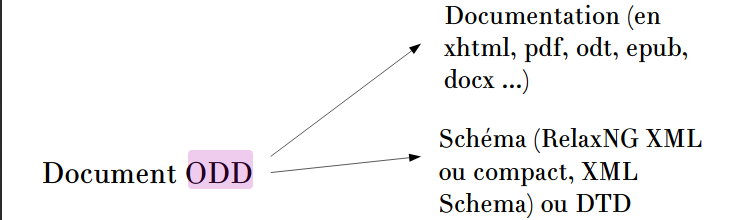
\includegraphics[width=16cm]{images/ODD.png}
    \label{ODD}
\end{figure}

\subsection{Créer l'ODD et l'associer à un document XML-TEI}

Un ODD est un document TEI. Pour ce qui est du projet Le Play, nous l'avons construit avec oXygen XML Editor. Pour faciliter sa construction, nous avons utilisé \emph{ODD By Example}\footnote{Pour plus d'informations sur le scénario \emph{oddbyexample}, voir Ariane Pinche, Séance 11, \inquote{Personnaliser son ODD}, Cours M2 TNAH, URL~: \url{https://github.com/ArianePinche/coursTNAH_XML-TEI/tree/master/seance11} (visité le 18/02/2020).}.

Après avoir installé notre scénario \emph{oddbyexample}, nous avons transformé l'0DD en RELAX NG, puis nous avons associé le schéma RELAX NG au fichier XML-TEI. Ainsi, l'association de l'ODD et du fichier XML-TEI se fait via le fichier RELAX NG. 

Une fois que notre fichier TEI est lié au schéma qui le contraint, il doit lui correspondre. Dès qu'un enchaînement de balises, contraint dans le schéma, n'est pas respecté, le fichier XML-TEI le signale : cela pousse donc à une certaine rigueur. Par ailleurs, si l'on a des doutes sur la façon d'encoder, on peut toujours se reporter à l'ODD qui explique les choix. Ainsi, si la personne qui encode se rend compte d'une erreur, elle peut modifier et mettre à jour l'ODD, en indiquant que c'est elle qui a fait la modification. 

\begin{figure}[ht]
    \centering
    \caption{Extrait de la table des matières de l'ODD pour le projet Le Play}
    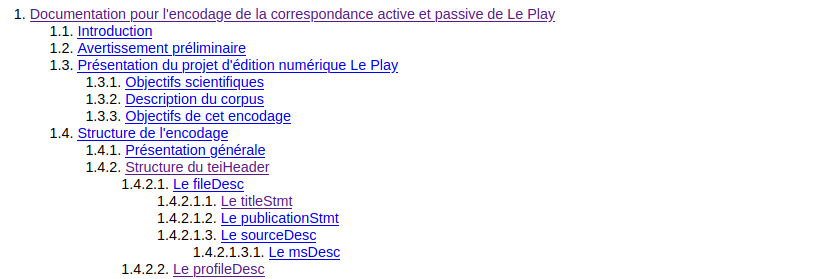
\includegraphics[width=16cm]{images/tableMatiereODD.png}
    \label{tableMatiereODD}
\end{figure}

\subsection{L'ODD dans nos projets}

Nous avons eu un rôle très différent quant à l'ODD pour nos deux projets. Pour ELICOM, l'ODD n'avait pas encore été réalisé. Nous n'avons donc été chargée que du travail en amont. En effet, avant de réaliser l'ODD, il faut avoir une connaissance assez large du corpus. Néanmoins, il a été parfois difficile pour nous de ne pas avoir d'ODD auquel nous pouvions nous référer pour garder une cohérence et une constance dans le choix des balises.

Pour le projet Le Play, c'est nous qui avons été chargée de la mise en place de l'ODD. Nous avons donc été au c\oe ur de certains choix. Néanmoins, il est à noter que cet ODD est encore perfectible. De nombreux cas n'ont pas encore été traités. C'est donc un document susceptible d'être modifié. Nous pensons notamment à l'encodage des documents joints à certaines lettres ainsi que nombre d'autres cas particuliers que nous n'avons pas eu le temps de traiter durant ce stage relativement court.
Il sera donc nécessaire de mettre l'ODD du CRHXIX à jour, au fil des cas particuliers rencontrés\footnote{Notre ODD pour le CRHXIX est joint à nos livrables.}.

L'ODD est donc un incontournable pour qui veut encoder des données en XML-TEI, de façon cohérente et pérenne.

XML a donc été le langage de base dont nous nous sommes servies pour nos éditions numériques de correspondance. Néanmoins, nous avons eu également recours à d'autres technologies.

\section{Au service d'XML}

\subsection{XSLT}

XSLT est un langage basé sur XML, permettant de styliser ou transformer des fichiers XML ou HTML. Comme nous l'avions déjà souligné dans la troisième partie\footnote{Voir 9.6.2 La question des \emph{tags}} nous aurions pu passer par une feuille de transformation pour passer du fichier XML-TEI exporté de Transkribus et criblé de fautes, à un fichier XML-TEI comportant les noms de balises conformes. Cela reste une possibilité mais pour notre part, nous n'avons pas poussé plus loin la réflexion. En revanche, nous avons eu recours au langage de programmation Python. 

\subsection{Python}

\subsubsection{Un \emph{script} Python pour extraire les fichiers XML}

Dans le cadre du projet ELICOM, Python nous a servi à extraire du résultat de l'OCR, le texte des différentes lettres pour les encoder en XML-TEI dans des fichiers séparés\footnote{Le \emph{script} Python sert à la fois à distinguer les lettres les unes des autres et à passer en TEI.}.

Pour cela, nous avons installé un environnement virtuel basé sur Python 3 avec plusieurs \emph{packages} dont \textbf{lxml} qui est un parseur pour les fichiers XML et HTML en Python, utilisé ici pour construire les fichiers XML,  ainsi que \textbf{beautifulsoup4} \inquote{qui permet une interaction simplifiée en Python avec les fichiers XML et HTML parsés}\footnote{Voir Alix Chagué, \emph{Ibidem}, p.85}. Par ailleurs, BeautifulSoup fonctionne sur les fichiers HTML mal formés, ce qui est le cas ici. Nous avons également importé le module \textbf{re} pour faire des regex dans Python.\\

Un \emph{script} Python avait déjà été réalisé par un membre de l'équipe du Labex OBVIL\footnote{Voir Fig. 10.11}. Nous avons donc eu un squelette commun, une base commune traitant les points communs aux différents corpus, mais à adapter à chacun. En effet, chaque corpus est tout de même à traiter différemment car les données n'apparaissent pas toujours de la même manière, à cause des différentes stratégies d'édition.

\begin{figure}[ht]
    \centering
    \caption{Extrait du \emph{script} \citecode{extraction-elicom.py}, capture d'écran de Sublime Text}
    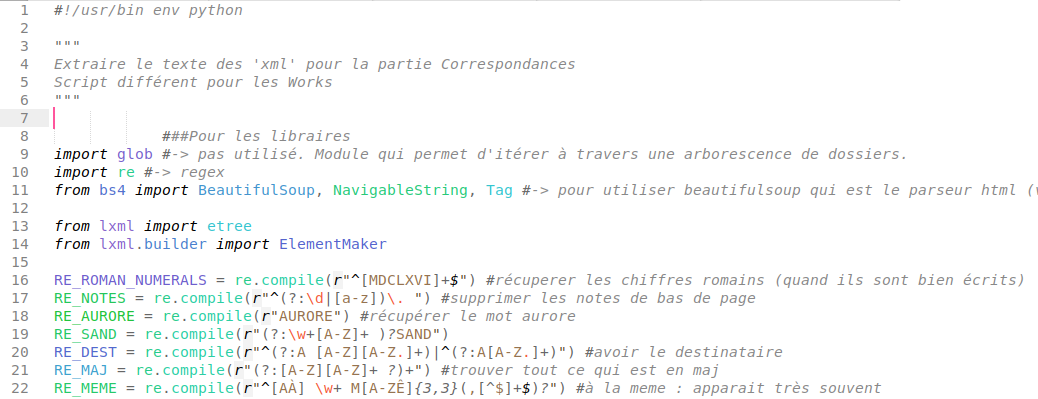
\includegraphics[width=15cm]{images/extraction.png}
    \label{extraction}
\end{figure}

\subsubsection{Les regex dans Python}

Avec les regex dans python, nous nous sommes surtout attachée à matcher les chiffres romains pour Lamartine, les chiffres arabes pour Lamennais, et les signatures pour Proudhon, afin de pouvoir extraire les lettres\footnote{Voir 8.2.5 Premiers repérages des marqueurs : pour Lamartine, les lettres sont toujours introduites par des chiffres romains, pour Lamennais par des chiffres arabes. Pour Proudhon, nous nous sommes servie de sa signature.}.

On peut constater sur la figure ci-dessus\footnote{Fig. 10.11} que les lettres de George Sand (\emph{script} \citecode{extraction-elicom.py}) ont été aussi extraites au moyen du repérage des chiffres romains via une regex.
\begin{figure}[ht]
    \centering
    \caption{Extrait du \emph{script} de Proudhon, capture d'écran de Github}
    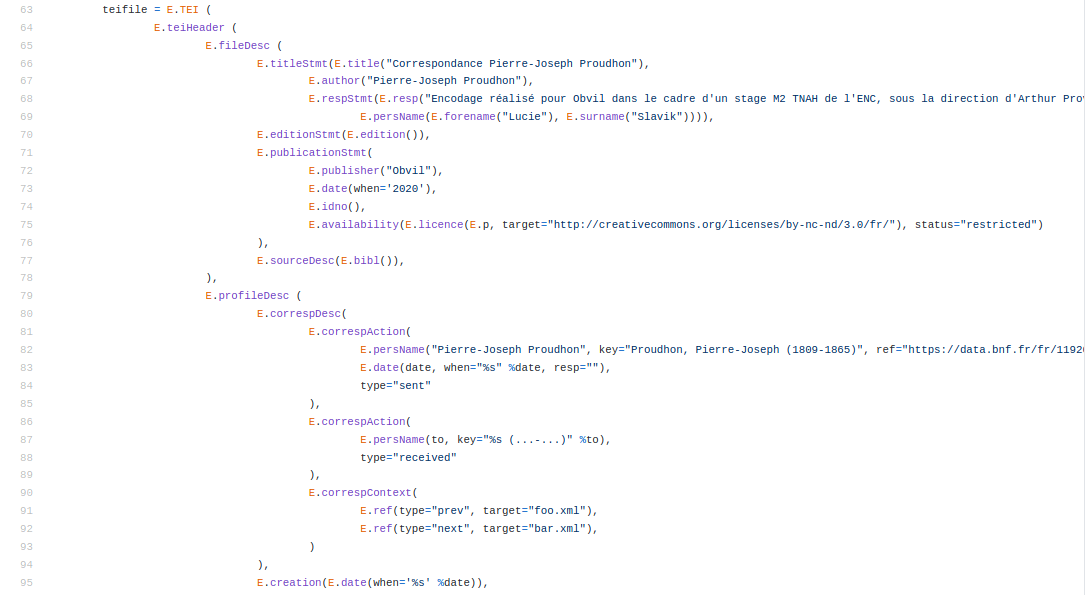
\includegraphics[width=15cm]{images/scriptProudhon.png}
    \label{scriptProudhon}
\end{figure}

Ainsi, à chaque chiffre arabe ou romain ou signature, une lettre était extraite et mise directement en XML-TEI grâce au module \textbf{lxml.builder}. La figure ci-dessous\footnote{Fig. 10.12} montre l'arborescence demandée depuis le \emph{script} Python de Proudhon.\\

Par ailleurs, nous nous sommes également servie des expressions régulières pour extraire les métadonnées et les récupérer ensuite dans le \citecode{<teiHeader>}. Par exemple, pour le \emph{script} de Proudhon, nous avons écrit \citecode{RE\_DEST = re.compile(r"A M\. [A-Z].+")} pour matcher les destinataires de Proudhon, et \citecode{RE\_DATE = re.compile(r"([\^,]+), (.+)\$")} pour matcher la date d'écriture de la lettre, puis nous avons mis ces informations dans le \citecode{<teiHeader>}\footnote{Voir les \emph{scripts} dans leur intégralité dans les livrables.}. 

\subsubsection{Les limites de l'OCR entravent l'efficacité du \emph{script} Python}

Cependant, tout n'est pas parfait du premier coup. Certes, Python nous avance beaucoup et fait gagner beaucoup de temps dans l'extraction des lettres et leur transformation en fichiers XML-TEI en vue de leur édition. Toutefois, certaines choses restent à modifier.

Tout d'abord, certaines modifications doivent parfois être faites en amont pour une meilleure extraction : c'est le cas lorsque des chiffres arabes ou romains ont été mal océrisés et empêchent la regex de les reconnaître : ainsi, les fautes de l'OCR rendent l'extraction difficile.

Par ailleurs, après l'application du \emph{script}, on remarque également certaines défaillances, encore dûes à la mauvaise océrisation. En effet, nous avons élaboré pour la correspondance de Lamennais une regex afin de matcher et supprimer les notes de bas de pages qui étaient disséminées au sein du texte. Des centaines de notes ont été ainsi supprimées. 
\begin{figure}[ht]
    \centering
    \caption{Lettre de Lamennais, notes mal matchées à cause de l'océrisation, \citecode{lamennais-cor-vol1-112.xml}}
    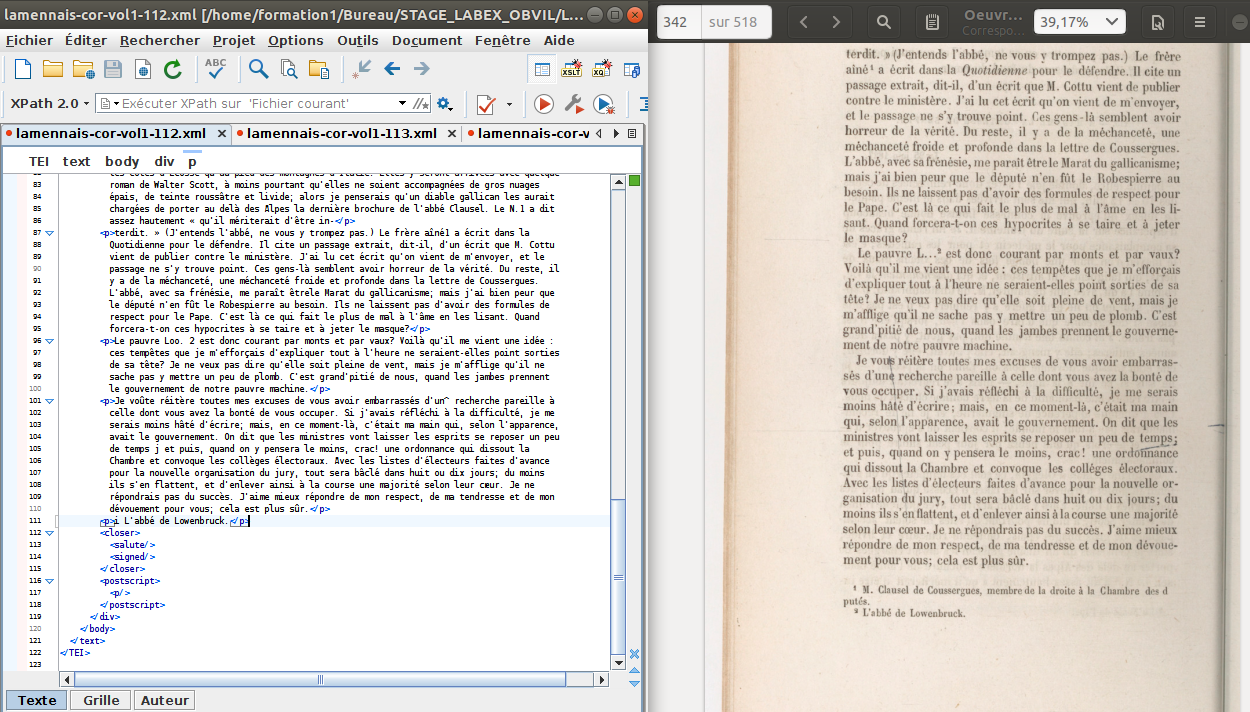
\includegraphics[width=16cm]{images/notesLamennais.png}
    \label{notesLamennais}
\end{figure}
Cependant, de nombreuses notes n'ont pas été matchées par la regex (et ont donc échappé à la suppression) car l'océrisation avait été mauvaise. L'exemple de la figure 10.13 est typique : on constate que la première note a été supprimée mais que la deuxième subsiste : le \inquote{2} a été pris pour un \inquote{i} par l'OCR. La note n'a donc pas été matchée et il faut donc la supprimer autrement\footnote{Pour notre part, nous l'avons fait manuellement.}.

Enfin, le résultat de l'OCR n'étant balisé que par des \citecode{<p>} et des \citecode{<span>}, et qu'aucune autre indication stylistique ou bien de structure n'apparaît, cela empêche un traitement plus fin des données pour la mise en page ou le signalement des vers. Ainsi, l'OCR ne tient pas compte des italiques, mais nous n'avons pas traité ce point. En revanche, pour ce qui est de la mise en page, nous nous sommes penchée sur la question : Lamartine surtout et parfois Lamennais glissaient des vers dans leurs lettres. Pour Lamartine, c'était assez fréquent. Il lui arrivait même parfois d'écrire une lettre intégralement en vers\footnote{La lettre 38 par exemple.}.

Afin de les remettre en valeur, nous avons choisi d'indiquer les strophes par les \citecode{<lg>} et les vers par les \citecode{<l>}, pour améliorer les repérages et la visualisation, dans le but de poursuivre l'objectif de cette édition numérique qui veut permettre une plus grande facilité d'accès au texte pour y effectuer des recherches plein texte et sur la structure, via l'interrogation des balises et des métadonnées.

Pour effectuer ce travail, nous avons dû mettre en regard les numérisations pour voir quelles lettres contiennent des vers. Nous avons donc fait ces ajouts manuellement.
\begin{figure}[ht]
    \centering
    \caption{Mise en place des \citecode{<lg>} et des \citecode{<l>} dans la correspondance de Lamartine}
    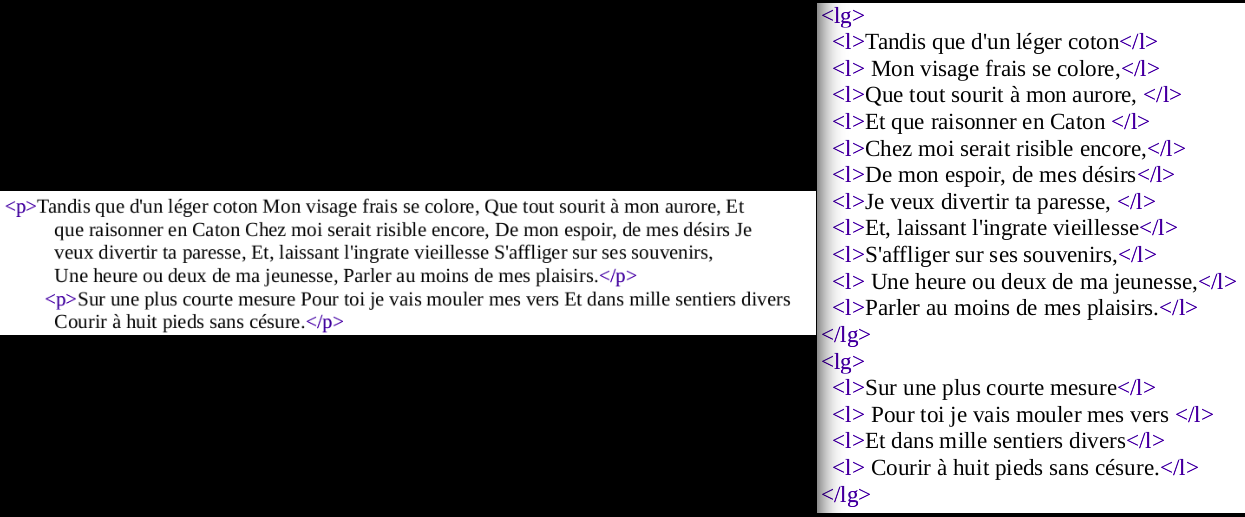
\includegraphics[width=16cm]{images/lamartineLG.png}
    \label{lamartineLG}
\end{figure}
On peut constater sur la figure 10.14 les modifications qui ont été faites. Sur la gauche, on voit le fichier XML qui a été extrait : les deux strophes apparaissent dans deux paragraphes (\citecode{<p>}), sans aucune distinction des vers. Sur la droite, les deux paragraphes sont devenus des strophes reconnues par les \citecode{<lg>}, et au sein des strophes, chaque vers (\citecode{<l>}) est marqué par un retour à la ligne.\\

XML est donc poussé au bout de ses possibilités avec l'apport d'autres technologies telles que Python, XSLT et les regex. Néanmoins, la qualité pas toujours optimale de l'OCR nécessite tout de même de nombreuses reprises à la fois techniques et orthographiques. 

Toutes ces technologies sont donc au service de l'édition numérique de correspondance et elles permettent de traiter les données acquises.



\chapter{Relever les défis du projet numérique}

\section{Des difficultés à surmonter}

Nous avions déjà évoqué plus haut\footnote{6.6 Le cahier des charges} les difficultés que rencontrent nombre de projets numériques, que cela soit dans le public ou le privé : deux tiers rencontrent de gros problèmes au cours de leur élaboration, et un tiers se solde par un échec\footnote{Voir Jean-Louis Foucard, Module de formation \inquote{Manager un projet Numérique} \inquote{Master Archives – Technologies numériques appliquées à l’histoire}, École Nationale des Chartes, mars 2020.}.

Nos deux projets n'échappent donc pas à cette constante. Pour ce qui est du projet au CRHXIX, nous pensons que le manque de subventions pourrait être un des freins au développement du projet, qui toutefois avance peu à peu. 

Pour ELICOM, nous n'avons pas assez de recul pour voir les difficultés que nous pourrions rencontrer. Une fois que l'ODD sera faite, ce sera bien-sûr un grand pas en avant, tant pour éclairer l'encodage que pour la pérennité des données.\\

Pour prévenir les difficultés, notre rôle en tant que stagiaire a été d'être un relais et d'assurer la transmission de notre travail, d'autant que nous avons réalisé la totalité de notre travail sur nos deux projets en télétravail. 

\section{Prévenir le \inquote{facteur d'autobus}}

Pour la réussite d'un projet, il s'agit d'éviter ce que les britanniques appellent le \emph{bus factor}, autrement dit, le \inquote{facteur d'autobus}, expression qui vient de la phrase \inquote{Combien de personnes clés dans votre équipe peuvent se faire renverser par un autobus avant que votre projet échoue ?}. Ainsi, \inquote{le ``facteur d'autobus'' est le nombre minimum de membres de l'équipe qui peuvent disparaître soudainement d'un projet avant que celui-ci ne s'arrête par manque de personnel compétent ou bien informé}\footnote{\emph{Facteur d'autobus}, Wikipédia, URL : \url{https://fr.wikipedia.org/wiki/Facteur_d\%27autobus} (visité le 28/09/2020).}.

Autrement dit, en tant que stagiaire, il faut qu'une fois que nous avons quitté le projet, les membres de l'équipe, que ce soit celle du CRHXIX ou du Labex OBVIL, aient en main tout notre travail et puisse profiter de ce que nous avons appris, compris, repris durant notre stage. Il s'agit d'assurer la transmission des savoirs et le transfert de compétences. 

\subsection{Les avantages de GitHub}

Pour cela, GitHub est un moyen intéressant pour le travail en équipe et la transmission. GitHub est un \inquote{service web d'hébergement et de gestion de développement de logiciels, utilisant le logiciel de gestion de versions Git}\footnote{\emph{GitHub}, Wikipédia, URL : \url{https://fr.wikipedia.org/wiki/GitHub} (visité le 28/09/2020).}. Il permet donc le versionnage\footnote{On entend par versionnage la \inquote{Gestion des différentes versions d'un même document}. Voir \cite{versionnage}} ainsi que le travail en équipe avec le partage de code.
Nous ne l'avons pas utilisé pour le projet Le Play mais pour le projet ELICOM\footnote{Voir OBVIL/Elicom, Github, URL : \url{https://github.com/OBVIL/elicom}}. Nous avons donc pu transmettre notre travail au fur et à mesure et faire des rapports au jour le jour pour une meilleur gestion de projet. À cela se sont ajoutés les appels réguliers avec le tuteur technique pour faire le point, et un rapport général en fin de stage.

Si nous n'avons pas usé de cette stratégie pour notre travail au CRHXIX, des contacts fréquents avec l'équipe, aussi bien par courriel que par téléphone ou encore par visioconférence ont eu lieu. Le transfert du travail se fera sous peu. Par ailleurs, pour le transfert de compétences, nous avons mis en place des tutoriels.

\subsection{Des tutoriels et des fiches de savoir pour assurer la transmission}

Ainsi, pour le CRHXIX, nous avons constitué divers tutoriels selon les technologies utilisées, afin que les membres de l'équipe puissent prendre la suite de la partie numérique.\\

Pour ce qui est de notre travail sur Transkribus, nous avons réalisé quatre tutoriels, pour chaque étape :

\begin{itemize}
    \item Un premier tutoriel pour le chargement des données et leur premier traînement\footnote{Voir dans les livrables \citecode{Tuto1\_preparation\_des\_donnees\_transkribus.pdf}}
    \item Un second dédié à l'entraînement du modèle \footnote{Voir dans les livrables \citecode{Tuto2\_entrainement\_du\_modele.pdf}}
    \item Un troisième consacré à l'application du modèle définitif \footnote{Voir dans les livrables \citecode{Tuto3\_application\_du\_modele.pdf}}
    \item Un quatrième qui traite de l'exportation des données depuis le serveur Transkribus \footnote{Voir dans les livrables \citecode{Tuto4\_exportation\_transkribus.pdf}}
\end{itemize}

Par ailleurs, nous avons réalisé un point sur notre travail pour dire où nous en étions et quelles conclusions nous tirions de cette première expérience\footnote{Voir dans les livrables \citecode{point\_transkribus.odt}}.\\

Pour ce qui est de notre travail sur XML-TEI et ODD, nous avons également travaillé à la transmission, pour le CRHXIX : 
\begin{itemize}
    \item Par la réalisation d'un tutoriel\footnote{Voir dans les livrables \citecode{Tuto\_XML-TEI\_CHRXIX.pdf}} pour la prise en main d'Oxygen XML Editor afin de réaliser les encodages
    \item Par la transmission d'un tutoriel sur l'ODD\footnote{Ce tutoriel n'a pas été réalisé par nos soins en revanche.}.
\end{itemize}
Par ailleurs, la documentation de l'ODD\footnote{L'ODD du CRHXIX est disponible dans les livrables.} est le moyen par excellence pour prévenir le \inquote{facteur d'autobus}. Nos choix y sont justifiés, et nos questionnements son présentés. Celui qui prendra la suite du projet pourra donc comprendre la logique de notre travail, perfectionner l'ODD et résoudre certains problèmes ou questionnements.

Quant à ELICOM, nous avons, au fur et à mesure de notre travail, constitué des fichiers rassemblant nos remarques sur l'HTML et le XML et à l'occasion du \emph{script} Python de chacun des auteurs. Nous y avons entre autres écrit quelques expressions régulières. Ces fichiers sont perfectibles et auraient pu être perfectionnés. Nous avons quand-même choisi de les mettre dans les livrables à titre d'exemple. À la fin de notre travail sur Lamartine, nous avons également réalisé un fichier récapitulatif sur le code Python.\begin{figure}[ht]
    \centering
    \caption{Rapport sur le code Python de Lamartine, capture d'écran de GitHub}
    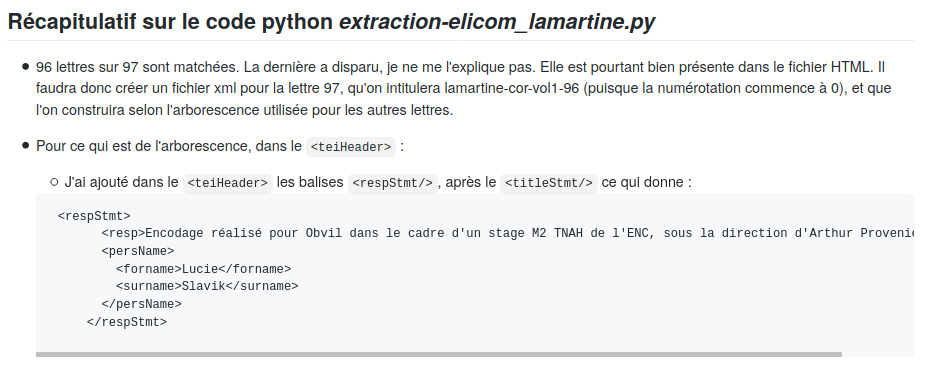
\includegraphics[width=16cm]{images/recapLamartine.png}
    \label{recapLamartine}
\end{figure}
Celui-ci est disponible sur GitHub\footnote{Voir \url{https://github.com/OBVIL/elicom/blob/master/extraction_cor_stage2020/cor_lamartine/remarques/recapitulatif_lamartine.md}}. La figure ci-dessus\footnote{Fig. 11.1} donne un échantillon de ce rapport rédigé au moyen du langage de balisage Markdown.\\

Par ailleurs, le cahier des charges du CRHXIX ayant été un peu détourné de sa fin en se transformant en rapport, il a toutefois permis également de faire un petit bilan de la situation pour voir où nous en étions et quelles étaient les prochaines étapes à suivre. \\

Enfin, nous avons réalisé des fiches pour accélérer certaines normalisations. Ainsi, pour le CRHXIX, nous avons écrit sept fiches pour les normalisations des index, que ce soit pour le recensement des correspondants dans le \citecode{<teiHeader>} ou les six index.

De même, pour ELICOM, nous avons constitué des index de correspondants pour pouvoir normaliser plus facilement chacun des destinataires lors des corrections des fichiers XML.

\subsection{Documenter son code}

Enfin, un des moyens d'assurer la transmission est la documentation du code en direct. En effet, pour ce qui est des \emph{scripts} Python pour ELICOM, nous avons essayé, du moins au début, de bien documenter notre code, à la fois pour mieux le comprendre et aussi pour mieux le faire comprendre. Cela fait partie des bonnes pratiques pour nos projets numériques. De même pour les premiers essais d'encodage en XML-TEI pour le CRHXIX, nous avons commenté chaque balise pour la justifier et l'expliquer. Nous avons été particulièrement attentive à cela dans un souci de transmission, et ceci nous a d'ailleurs aidée nous-même au moment de la rédaction de l'ODD car il n'y avait plus qu'à suivre les indications déjà présentes dans les fichiers XML commentés au fur et à mesure.\\


Nous avons donc tenté de relever au cours de nos stages les défis de ces deux projets d'édition numérique de correspondance sur des corpus du XIX\up{e} siècle. Cette partie de traitement des données s'est réalisée autour du langage XML, avec le souci de transmettre non seulement les réalisations de notre travail mais également les étapes de réflexion par lesquelles nous sommes passée.
